% [H] means put the figure HERE, directly when you input this code.
\begin{figure}[H]
	\centering
	\captionsetup{width=1.0\linewidth}

% We set the width of the figure based on the width of one line of text on the page.
% The value can be tuned to any value in [0.0, 1.0] to scale the image while maintaining its aspect ratio.

	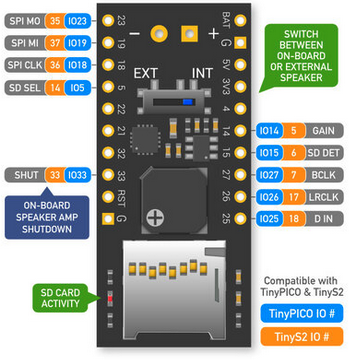
\includegraphics[width=0.75\linewidth]{graphics/audioshield_pinouts.png}

% Caption is defined with a short and long version. The short version is shown in the
% List of Figures section, and the long version is used directly with the figure.
	\caption[I2S Audio Shield Pinouts]{An illustration of the I2S audio shield pinouts provided by \cite{unexpected_maker}}

% For figures label should be defined after the caption to ensure proper figure numbering.
	\label{fig:audioshield_pinouts}

\end{figure}